\documentclass{article}

\usepackage{tikz}
\usetikzlibrary{shapes,arrows, positioning}


\begin{document}

\section{Drawing the figures (using loops)}

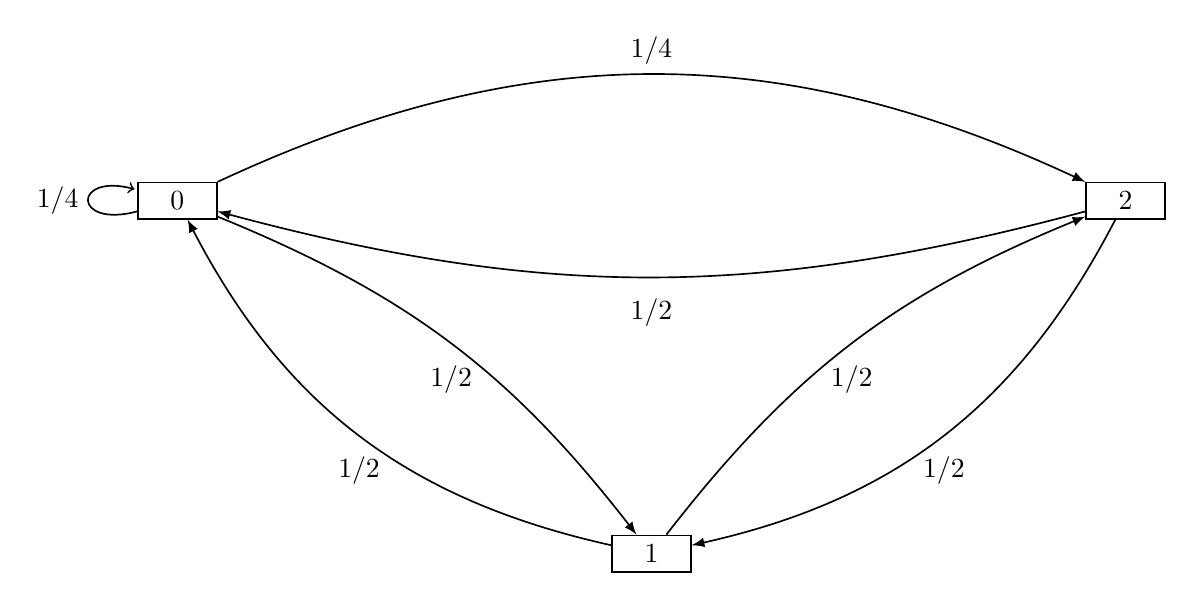
\begin{tikzpicture}[-latex,node distance =4cm and 5cm,semithick,
state/.style={rectangle, draw, minimum width=1cm}] % here all the outputs are recangle so i can use them as a preedefine them,here state is my rectangle,  and 4cm is vertical distance, and 5cm is horizontal distance. 
\node[state](C){1};% we define 1st node here, now instead of writing the circle ... rectangle, now all this rectangle  i have written in form of state, so i can write them as a state, so i can write them as a state of c, so that is of the 1. and here c is nothing but my label.
\node[state](A)[above left=of C]{0};
\node[state](B)[above right=of C]{2};

%How we can define the self loop?

\path(A)edge[loop left]node[left]{1/4}(A); % start from A and ending at A, and loop left 
\path(C)edge[bend left =25]node[below=0.15cm]{1/2}(A); %here loop bend at the left, and left of the 25 degree,
\path(A)edge[bend right =-15]node[below =0.15cm]{1/2}(C); % starting from A and ending at C, this is right side,  
\path(A)edge[bend left =25]node[above]{1/4}(B);
\path(B)edge[bend left =15]node[below =0.15cm]{1/2}(A);
\path(C)edge[bend left =15]node[below =0.15cm]{1/2}(B);
\path(B)edge[bend right =-25]node[below =0.15cm]{1/2}(C);

\end{tikzpicture}
\end{document}

